\documentclass[12pt,a4paper]{article}
\usepackage{styles}

\lstset{style=sharpc, tabsize=1}

\renewcommand{\sectionbreak}{\clearpage}

\newcommand{\texta}{Stärken\\[-1ex]}
\newcommand{\textb}{Schwächen\\[-1ex]}
\newcommand{\textcn}{Chancen\\[-1ex]}
\newcommand{\textdn}{Risiken\\[-1ex]}

\author{Alexander van Schie \& Oli Dias}
\title{Gruppenarbeit 3 - Abschliessende Analyse des Providers und Cloud Application Design}
\begin{document}
\maketitle
\newpage
\tableofcontents
\newpage
\section{Analyse Service Level Agreegment (SLA)}
\begin{itemize}
    \item 1. Es wird eine etwas andere Art von SLO’s gemacht, nämlich wird das Problem nach Schwerheitsgrad klassifiziert und je schlimmer es ist, desto schneller muss RedHat reagieren (https://access.redhat.com/support/offerings/openshift/sla)
    \item 2.
    \item 3. Generell werden keine Metriken oder Messwerte erwähnt. Vielmehr werden Probleme zusammengefasst und nach Schwerheitsgrad klassifiziert. (https://www.openshift.com/legal/terms/)
    \item 4. Je nach SLA müssen verschieden Dinge eingehalten werden. Was mir persönlich als wichtig erscheint ist eine Vereinbarung bezüglich dem Kundensupport innerhalb einer gewissen Zeit da (a) ein Unterbruch meiner Applikation je nachdem grosse Konsequenzen für mein Unternehmen haben kann. Grundsätzlich sollte ein Cloud-Provider ausgewählt werden, der quasi to big to fail ist (b).
    \item 5. Je nach Branch muss man sich mit den Datenschutzbestimmungen des Cloud Providers auseinander setzen. Beispielsweise wäre es für Banken nicht gerade ideal, Kundendaten auf ausländische Server zu migrieren/verwalten
\end{itemize}

\section{Hands-On Lakeside Mutual}
Die zu deployenden Komponenten lassen sich in zwei Kategorien einteilen; Frontend und Backend. Das Setup der beiden Teile des Backends werden im nachfolgenden Unterkapitel besprochen, das Frontend im Unterkapitel \ref{subsec:frontend}. 

\subsection{Spring Boot Backend Setup}
Für das Migrieren des Backends der Lakeside Mutual DDD Applikation eignet sich für die beiden Komponenten Customer-Core und Customer-Management-Backend ein Wildfly Projekt auf Openshift. Dies sollte analog wie schon beim Deployment der Self-Information Applikation funktionieren, da alle drei Applikationen Spring Boot verwenden. 

Dazu sind folgende Schritte notwendig:
\begin{enumerate}
	\item Hinzufügen der \texttt{.s2i/bin/run} Datei in beiden Spring Boot Apps, die den Befehl für das Ausführen des gebuildeten Jar Files enthält:
	\begin{lstlisting}
	exec java -jar /wildfly/standalone/deployments/
	 customer-management-backend-0.0.1-SNAPSHOT.jar
	\end{lstlisting}
	\item Anpassen der Application-Properties in Customer-Management-Backend: 
	\begin{itemize}
		\item Property \texttt{customercore.baseURL} auf die URL des Customer Cores einstellen. Diese ist sichtbar gemäss Abbildung \ref{fig:os-routes} in Openshift Cloud herauszufinden. 
		\item Property \texttt{server.port} aus derselben Übersicht auslesen und setzen (Default 8080)
	\end{itemize}
	\item Anpassen der Application-Properties in Customer-Core:
	\begin{itemize}
		\item Property \texttt{server.port} setzen (Default 8080)
	\end{itemize}
\end{enumerate}

\begin{figure}[h]
	\centering
	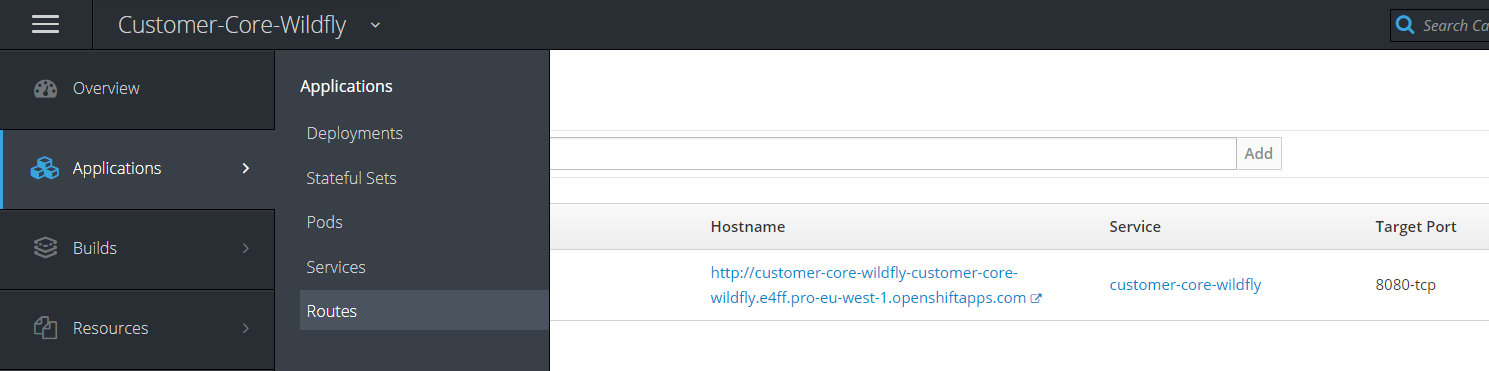
\includegraphics[width=1\linewidth]{img/os-routes}
	\caption{Navigation zu Routes}
	\label{fig:os-routes}
\end{figure}

Da Customer-Management-Backend von der Komponente Customer-Core abhängig ist, muss Customer-Core zuerst deployt werden. Ansonsten wirft die Applikation eine Laufzeit-Exception, da keine Verbindung zum Core hergestellt werden kann. 

\subsection{Frontend Deployment}\label{subsec:frontend}
Openshift bietet Node.js Projekte an, welches sich für die React App eignet. 

Nachdem das Nodejs-Projekt erstellt und das GitHub-Repository erstellt ist, beginnt ein zuständiger Pod gleich mit dem Build. Unglücklicherweise wurde mit unserem Setup an dieser Stelle der Build unterbrochen aufgrund von Limiten, die unsere Subscription setzt. Da das Frontend aber von beiden anderen Komponenten abhängig ist, bleibt uns nichts anderes übrig, als die Frontend-Komponente lokal auszuführen. 

\begin{figure}[h]
	\centering
	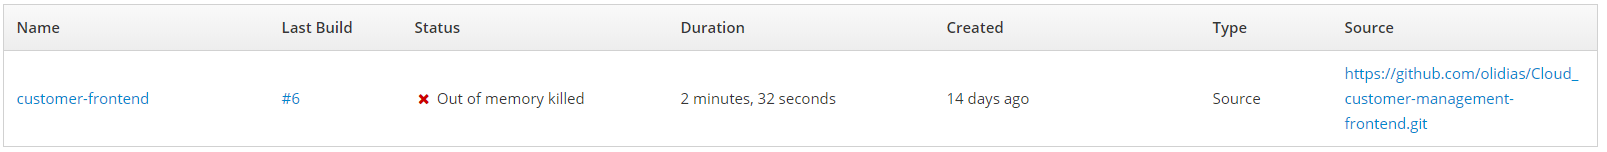
\includegraphics[width=1\linewidth]{img/os-frontend-build-fail}
	\caption{Build-Failure aufgrund von Memory-Limiten}
	\label{fig:os-frontend-build-fail}
\end{figure}

Für die lokale Ausführung wird Nodejs benötigt. Ist dies installiert, ist noch eine zusätzliche Konfiguration nötig: Wir müssen auf das Management-Backend zugreifen können und dafür die URL anpassen. Wie im vorgehenden Kapitel schon erwähnt, findet man den URL des Management-Backends in dessen Projekt auf Openshift unter Applications $\rightarrow$ Routes. Die URL muss im File \texttt{src/config.js} angepasst werden:
\begin{lstlisting}[showstringspaces=false]
export const customerManagementBackend =
 getEnvironmentVariable(
  "REACT_APP_CUSTOMER_MANAGEMENT_BACKEND",
  "http://customer-management-backend.e4ff.
    pro-eu-west-1.openshiftapps.com/"
)
\end{lstlisting}
Sind diese Schritte durchgeführt, kann die WebApp mit \texttt{npm start} ausgeführt werden. Es sollte automatisch der Browser mit dem Frontend aufgerufen werden. 

Mit dem erläuterten Setup hat das Frontend wie gewünscht funktioniert, sogar mit dem Chat, dessen History nach einem Neustart immernoch vorhanden war. 

\subsection{Herausforderungen}
\section{Hands-On Persistence}


\section{Twelve-Factor Apps}
    \begin{table}[h]
        \begin{tabular}{ll}
        \multicolumn{2}{l}{Engineering Projekt (Waitless)} \\
        Erfüllt               & Nicht erfüllt              \\
        Codebase              & Disposability              \\
        Dependencies          & Dev/prod parity            \\
        Config                & Logs                       \\
        Backing services      & Admin processes            \\
        Build, release, run   &                            \\
        Processes             &                            \\
        Port binding          &                            \\
        Concurrency           &                            \\
        Port binding          &                            \\
        \end{tabular}
    \end{table}

\subsection{Anpassungen}
    \begin{itemize}
        \item Disposability:
        \item Dev/prod parity: Die ganze Applikation wurde nur auf einem System entwickelt. Sobald Code eingecheckt und die Tests
              erfolgreich waren, war der Code bereits produktiv.
        \item Logs: Das Verhalten der Applikation wurde mit Enduser-Tests überprüft. Mit der Implementation von Logs werden alle
              Informationen festgehalten.
        \item Admin processes:
    \end{itemize}

\section{Security Features und Assessment}

In den Terms und Conditions von Openshift ist ganz klar zu entnehmen, dass der Anwedender für Themen des Datenschutzes die Verantwortung übernimmt.
So hat der Anwender sicherzustellen, dass die Daten der Anwender seiner Applikation geschützt werden. Dies beinhaltet die Implementation von
Datnschutzrichtlinien, welche rechtlich abgestimmt sind. Zudem müssen die Anwender darüber informiert werden, dass ihre Daten auf der Infrstruktur
von Red Hat abgelegt wird und sie dem somit zustimmen.

Red Hat gibt bekannt, dass folgende Technologien von ihrem PaaS unterstützt werden:

\begin{itemize}
    \item SELinux
    \item Process, network, and storage separation
    \item Stateful and stateless inspection firewall
    \item Proactive monitoring of capacity limits
    \item Intrusion detection
    \item Port monitoring
    \item Pam namespace
    \item Security compliance frameworks
    \item RPM verification and vulnerabilities updated
    \item Remote logging
    \item Encrypted communications
\end{itemize}
https://www.openshift.com/policy/security/

\subsection{Checkliste Security Assessment}
1. Encrypted Communication/ (Security) -> 10
Openshift nutzt Kubernetes und die Kommunikation bei Kubernetes ist standardmässig mit TLS verschlüsselt.


2. Backups -> 3
Backups müssen selbst gemacht werden, es gibt hierfür keinen Service. Positive ist jedoch, dass das Vorgehen dokumentiert ist.


3. Location -> 5
Openshift wird vermutlich Data Centers an mehreren geographischen Standorten haben, kommuniziert dies jedoch nicht öffentlich.


4. Server Redundancy (Data Centre Physical Security, Disaster Tolerance) -> 8
Da Openshift mit Kubernetes arbeitet, besteht auch die Möglichkeit der Nutzung von Replicas, diese müssen jedoch selbst definiert werden.


5. Service Authentification (for Administration stuff) -> 10
Authentifizierungserfahren laufen über OAuth und bietet alle gängigen Möglichkeiten (\url{https://docs.openshift.com/enterprise/3.0/admin_guide/configuring_authentication.html})


6. Appropriate SLA (with Incident Handling) -> 7
Es gibt ein SLA, in dem wichtige Punkte zur Einhaltung der Servicebedingungen festgehalten sind. Was jedoch nicht zu entnehmen ist, sind Strafen, die bei Nichteinhaltung fällig werden.


7. Data Isolation (Customer based, Data Integrity)
Kubernetes NetworkPolicy wird voll unterstützt und Projekte können ebenfalls in einer isolierten Umgebung betrieben werden.


8. Transparency (Monitoring) -> 8
Quotas sowie laufende Prozesse können eingesehen werden


9. Network design und Logging -> 5
Standardmässig werden Logs geschrieben, diese waren unserer Erfahrungen nach unzureichend (was das Fehlerhandling erschwerte)


\section{SWOT-Assessment von Cloud Provider und Cloud Offering}

\begin{tikzpicture}[font=\small,
        any/.style={draw, text width=.5\linewidth-1cm, align=center,               anchor=center, inner sep=5pt},
        row 1/.style={nodes={any, minimum height=1cm, fill=black!10}},
        row 2/.style={nodes={any, minimum height=9cm}},
        row 3/.style={nodes={any, minimum height=8cm}},
        row 2 column 1/.style={nodes={any, minimum height=1cm, fill=black!10, rotate=90, minimum width=9cm}},
        row 3 column 1/.style={nodes={any, minimum height=1cm, fill=black!10, rotate=90, minimum width=8cm}}
    ]
    \matrix (SWOT) [matrix of nodes, inner sep=0pt,
    column sep=-1\pgflinewidth,
    row sep=-1\pgflinewidth,
    inner sep=0pt]
    {
     & {\texta} & {\textb} \\
     {\textcn} & \begin{itemize}
        \item Web App Design
        \item Einfache Projektinitialisierung
        \item Command Line Interface (CLI)
    \end{itemize} &\begin{itemize}
        \item Limitierte Ressourcen
        \item Limitierete Projektauswahl
        \item Limitierte Abonnemente
        \item Preis
        \item Web App Struktur ?
    \end{itemize} \\
     {\textdn} & \begin{itemize}
        \item Nutzung von Kubernetes
        \item Ausbaubare Service Dokumentation
        \item Chance zur Änderung (Nicht to big to change)
    \end{itemize} & \begin{itemize}
        \item Transparenz Fehlerbehandlung
        \item Transparenz Nutzungsbedingungen
        \item Ablehnung jeglicher Sicherheitsaspekte
        \item Kleine Community
    \end{itemize} \\
    };
    \node[below right =1mm of SWOT.south west] {S indicates standardization ongoing activities};
    \draw[fill=black!10] ($(SWOT-1-2.north west)+(\pgflinewidth/2,-\pgflinewidth/2)$) rectangle ($(SWOT-1-3.north east)+(-\pgflinewidth/2,-\pgflinewidth/2+1cm)$)
        node[midway] {Interne Analyse};
    \draw[fill=black!10] ($(SWOT-3-1.north west)+(-1cm+\pgflinewidth/2,\pgflinewidth/2)$) rectangle ($(SWOT-2-1.north east)+(\pgflinewidth/2, -\pgflinewidth/2)$)
        node[midway, rotate=90] {Externe Analyse};
    \end{tikzpicture}

\section{Provider Evaluation Checkliste}
    \begin{table}[]
        \begin{tabular}{lll}
            Kriterium & Erfüllt & Kommentar                                                                                 \\
            Umfangreicher Technologiekatalog & Jein & Welches Angebot stellt uns der Anbieter zur Verfügung.                \\
            Unternehmungsgrösse des Anbieters & Nein & Grosse Unternehmen haben tendenziel mehr Erfahrung als Cloud Anbieter\\
            Customizing & Jein & Ist es möglich, Ressourcen nach beliebigem Bedarf zu skalieren?                            \\
            Dokumentation & Ja &                                                                                            \\
            Community & Nein & Gibt es eine Community, die bei häufigen Problemen helfen kann?                              \\
        \end{tabular}
    \end{table}

\section{Management Summary}

\end{document}